\documentclass[aspectratio=169]{beamer}
\usepackage[utf8]{inputenc}
\usepackage[T1]{fontenc}
\usepackage{listings}
\usepackage{xcolor}
\usepackage{tikz}

% Tema
\usetheme{Madrid}
\usecolortheme{default}

% Configuración de colores para código
\definecolor{codegreen}{rgb}{0,0.6,0}
\definecolor{codegray}{rgb}{0.5,0.5,0.5}
\definecolor{codepurple}{rgb}{0.58,0,0.82}
\definecolor{backcolour}{rgb}{0.95,0.95,0.92}

% Estilo para código
\lstdefinestyle{mystyle}{
    backgroundcolor=\color{backcolour},
    commentstyle=\color{codegreen},
    keywordstyle=\color{blue},
    numberstyle=\tiny\color{codegray},
    stringstyle=\color{codepurple},
    basicstyle=\ttfamily\footnotesize,
    breakatwhitespace=false,
    breaklines=true,
    captionpos=b,
    keepspaces=true,
    numbers=left,
    numbersep=5pt,
    showspaces=false,
    showstringspaces=false,
    showtabs=false,
    tabsize=2,
    frame=single,
    rulecolor=\color{black},
    escapeinside={(*@}{@*)}
}

\lstset{style=mystyle}

% Configuración adicional para evitar problemas con fragile
\makeatletter
\newenvironment{code}{\begin{lrbox}{\@tempboxa}\begin{minipage}{\textwidth}}{\end{minipage}\end{
lrbox}\usebox{\@tempboxa}}
\makeatother

% Información del documento
\title{Introducción a Git y GitHub}
\subtitle{Control de versiones para desarrolladores}
\author{M.C. Edwin Enrique Pérez Rodríguez \\ Dr. Juan Carlos Cajas García}
\institute{ENES Mérida}
\date{\today}

\begin{document}

% Portada
\frame{\titlepage}

% Tabla de contenidos
\begin{frame}
\frametitle{Contenido}
\tableofcontents
\end{frame}

% Sección 1: ¿Qué es Git?
\section{¿Qué es Git?}
\begin{frame}
\frametitle{¿Qué es Git?}
\begin{itemize}
    \item \textbf{Sistema de control de versiones distribuido}
    \item Creado por Linus Torvalds en 2005
    \item Permite rastrear cambios en archivos y coordinar trabajo entre múltiples personas
    \item Características principales:
    \begin{itemize}
        \item Rápido y eficiente
        \item Distribuido (cada desarrollador tiene una copia completa del historial)
        \item Soporte para desarrollo no lineal (ramas)
        \item Gratuito y de código abierto
    \end{itemize}
\end{itemize}
\end{frame}

\begin{frame}
\frametitle{¿Por qué usar Git?}
\begin{columns}
\column{0.5\textwidth}
\textbf{Ventajas:}
\begin{itemize}
    \item Historial completo de cambios
    \item Trabajo colaborativo
    \item Experimentación segura (ramas)
    \item Reversión de cambios
    \item Respaldo distribuido
\end{itemize}

\column{0.5\textwidth}
\begin{center}
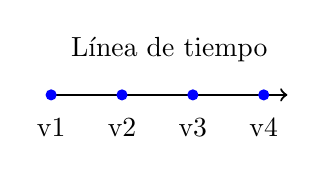
\begin{tikzpicture}[scale=0.6]
    \draw[thick, ->] (0,0) -- (5,0);
    \foreach \x in {0,1.5,3,4.5}
        \filldraw[blue] (\x,0) circle (3pt);
    \node[below] at (0,-0.3) {v1};
    \node[below] at (1.5,-0.3) {v2};
    \node[below] at (3,-0.3) {v3};
    \node[below] at (4.5,-0.3) {v4};
    \node[above] at (2.5,0.5) {Línea de tiempo};
\end{tikzpicture}
\end{center}
\end{columns}
\end{frame}

\begin{frame}
\frametitle{Los tres estados de Git}
Git tiene tres estados principales en los que pueden estar tus archivos:

\begin{enumerate}
    \item \textbf{Modified (Modificado):} Has cambiado el archivo pero aún no lo has confirmado
    \item \textbf{Staged (Preparado):} Has marcado el archivo modificado para ir en tu próximo commit
    \item \textbf{Committed (Confirmado):} Los datos están almacenados de forma segura en tu repositorio local
\end{enumerate}

\vspace{0.5cm}
Esto nos lleva a las tres secciones principales de un proyecto Git:
\begin{itemize}
    \item Working Directory (Directorio de trabajo)
    \item Staging Area (Área de preparación)
    \item Git Directory (Repositorio)
\end{itemize}
\end{frame}

% Sección 2: ¿Qué es GitHub?
\section{¿Qué es GitHub?}
\begin{frame}
\frametitle{¿Qué es GitHub?}
\begin{itemize}
    \item \textbf{Plataforma de alojamiento de código}
    \item Basada en Git
    \item Funcionalidades adicionales:
    \begin{itemize}
        \item Repositorios remotos
        \item Colaboración (Pull Requests, Issues)
        \item Revisión de código
        \item GitHub Actions (CI/CD)
        \item GitHub Pages (hosting de sitios web)
        \item Control de acceso y permisos
    \end{itemize}
    \item Alternativas: GitLab, Bitbucket, Gitea
\end{itemize}
\end{frame}

\begin{frame}
\frametitle{Git vs GitHub}
\begin{center}
\begin{tabular}{|p{5cm}|p{5cm}|}
\hline
\textbf{Git} & \textbf{GitHub} \\
\hline
Sistema de control de versiones & Servicio de hosting \\
\hline
Software local & Plataforma web \\
\hline
Línea de comandos & Interfaz gráfica \\
\hline
Gratuito y open source & Gratuito con planes de pago \\
\hline
Funciona sin internet & Requiere internet \\
\hline
\end{tabular}
\end{center}
\end{frame}

% Sección 3: Instalación
\section{Instalación de Git}
\begin{frame}[fragile]
\frametitle{Instalación en Windows}
\begin{enumerate}
    \item Descargar desde: \texttt{https://git-scm.com/download/win}
    \item Ejecutar el instalador
    \item Opciones recomendadas:
    \begin{itemize}
        \item Use Git from the command line.
        \item Use the OpenSSL library.
        \item Checkout Windows-style, commit Unix-style line endings.
    \end{itemize}
    \item Verificar instalación:
\end{enumerate}

\begin{lstlisting}[language=bash, caption=Verificar versión de Git]
git --version
\end{lstlisting}

Salida esperada: \texttt{git version 2.x.x}
\end{frame}

\begin{frame}[fragile]
\frametitle{Instalación en Linux}
\textbf{Ubuntu/Debian:}
\begin{lstlisting}[language=bash]
sudo apt update
sudo apt install git
\end{lstlisting}

% \textbf{Fedora:}
% \begin{lstlisting}[language=bash]
% sudo dnf install git
% \end{lstlisting}
%
% \textbf{Arch Linux:}
% \begin{lstlisting}[language=bash]
% sudo pacman -S git
% \end{lstlisting}

\textbf{Verificar instalación:}
\begin{lstlisting}[language=bash]
git --version
\end{lstlisting}
\end{frame}

% Sección 4: Configuración
\section{Configuración de Git}
\begin{frame}[fragile]
\frametitle{Configuración inicial}
\textbf{Configurar nombre de usuario:}
\begin{lstlisting}[language=bash]
git config --global user.name "Tu Nombre"
\end{lstlisting}

\textbf{Configurar correo electrónico:}
\begin{lstlisting}[language=bash]
git config --global user.email "tu@email.com"
\end{lstlisting}

\textbf{Configurar editor por defecto (opcional):}
\begin{lstlisting}[language=bash]
git config --global core.editor "vim"
git config --global core.editor "code --wait"
git config --global core.editor "nano"
\end{lstlisting}
\end{frame}

\begin{frame}[fragile]
\frametitle{Ver configuración}
\textbf{Ver toda la configuración:}
\begin{lstlisting}[language=bash]
git config --list
\end{lstlisting}

\textbf{Ver configuración específica:}
\begin{lstlisting}[language=bash]
git config user.name
git config user.email
\end{lstlisting}

\textbf{Ver ubicación de archivos de configuración:}
\begin{lstlisting}[language=bash]
git config --list --show-origin
\end{lstlisting}
\end{frame}

% Sección 5: Comandos principales
\section{Comandos principales de Git}
\begin{frame}[fragile]
\frametitle{Crear un repositorio}
\textbf{Inicializar un nuevo repositorio:}
\begin{lstlisting}[language=bash]
mkdir mi-proyecto
cd mi-proyecto
git init            "Iniciar rastreo de cambios."
\end{lstlisting}

\textbf{Verificar estado:}
\begin{lstlisting}[language=bash]
git status      "Ver cambios realizados hasta el momento."
\end{lstlisting}
\end{frame}

\begin{frame}[fragile]
\frametitle{Agregar y confirmar cambios}
\textbf{Agregar archivos al área de staging:}
\begin{lstlisting}[language=bash]
git add archivo.txt "Agregar un archivo en especifico"
git add .           "Agregar todos los archivos que fueron modificados."
git add *.py        "Agregar los cambios realizados en todos los archivos"
                    "que terminen en .py"
\end{lstlisting}

\textbf{Confirmar cambios (commit):}
\begin{lstlisting}[language=bash]
git commit -m "Mensaje descriptivo del cambio"
git commit -am "Mensaje del commit (para nuevos cambios hechos a un commit"
               "reciente)."
\end{lstlisting}
\end{frame}

\begin{frame}[fragile]
\frametitle{Ver historial}
\textbf{Ver historial de commits:}
\begin{lstlisting}[language=bash]
git log             "Enlista todos los commits realizados."
git log --oneline   "Muestra el commit mas reciente."
git log -n 5        "Enlista los ultimos 5 commits mas recientes."
\end{lstlisting}

\textbf{Ver diferencias:}
\begin{lstlisting}[language=bash]
git diff archivo.extension          "Muestra los cambios que NO estan en el"
                                    "staging area. Cambios que aun no has"
                                    "agregado con git add"

git diff --staged archivo.extension "Muestra los cambios que SI estan en el"
                                    "staging area. Cambios ya agregados"
                                    "con git add."
\end{lstlisting}
\end{frame}

\begin{frame}[fragile]
\frametitle{Trabajar con ramas}
\textbf{La Rama Main}

La rama main es la rama principal del proyecto. Es como el "tronco" del árbol:

    \begin{itemize}
        \item Representa el código que está en producción o listo para producción
        \item Es la rama por defecto cuando clonas o creas un repositorio
        \item Generalmente contiene código probado y funcional
        \item Es donde finalmente se integran todos los cambios aprobados
    \end{itemize}

    Buena práctica: Nunca trabajes directamente en main. Protégela para evitar errores accidentales.
\end{frame}

\begin{frame}[fragile]
    Subramas (Feature Branches / Ramas de trabajo)
    Las subramas son ramas temporales que se crean desde main para trabajar en:

    \begin{itemize}
        \item Nuevas funcionalidades
        \item Correcciones de bugs
        \item Experimentos
        \item Desarrollo individual
    \end{itemize}

\textbf{Crear y cambiar ramas:}
\begin{lstlisting}[language=bash]
git branch  "Enlista todas las ramas del repositorio."
git branch nueva-funcionalidad  "Crea una nueva rama."
git checkout nueva-funcionalidad    "Cambiar a la rama llamada: 
                                    "nueva-funcionalidad."
\end{lstlisting}

% \textbf{Fusionar ramas:}
% \begin{lstlisting}[language=bash]
% git checkout main
% git merge nueva-funcionalidad
% \end{lstlisting}
\end{frame}

\begin{frame}[fragile]
\frametitle{Deshacer cambios}
% \textbf{Descartar cambios no confirmados:}
% \begin{lstlisting}[language=bash]
% git checkout -- archivo.txt
% git checkout -- .
% \end{lstlisting}

    \textbf{Deshacer cambios del staging area:}
\begin{lstlisting}[language=bash]
git restore archivo.extension
\end{lstlisting}

% \textbf{Revertir un commit:}
% \begin{lstlisting}[language=bash]
% git revert HEAD
% git reset --hard <hash-commit>
% \end{lstlisting}
\end{frame}

% Sección 6: GitHub
\section{Descargar repositorios de GitHub}
\begin{frame}[fragile]
\frametitle{Clonar un repositorio}
\textbf{Clonar repositorio completo:}
\begin{lstlisting}[language=bash]
git clone <url-del-repositorio>
git clone https://github.com/usuario/repositorio.git

"Clonar repositorio a carpeta especifica."
git clone https://github.com/usuario/repo.git mi-carpeta 
\end{lstlisting}

\textbf{Clonar rama específica:}
\begin{lstlisting}[language=bash]
git clone -b nombre-rama https://github.com/usuario/repo.git
\end{lstlisting}
\end{frame}

\begin{frame}[fragile]
\frametitle{Trabajar con repositorios remotos}
\textbf{Ver repositorios remotos:}
\begin{lstlisting}[language=bash]
git remote -v
\end{lstlisting}

\textbf{Agregar repositorio remoto:}
\begin{lstlisting}[language=bash]
git remote add origin https://github.com/usuario/repo.git
\end{lstlisting}

\textbf{Subir cambios (push):}
\begin{lstlisting}[language=bash]
git push -u origin main
git push
\end{lstlisting}

\textbf{Descargar cambios (pull):}
\begin{lstlisting}[language=bash]
git pull origin main
\end{lstlisting}
\end{frame}

\begin{frame}[fragile]
\frametitle{Flujo de trabajo completo}
\begin{lstlisting}[language=bash]
git clone https://github.com/usuario/proyecto.git
cd proyecto

"Si se trabaja en otra rama que no se la main"
git checkout -b mi-funcionalidad

git add .
git commit -m "Agregar nueva funcionalidad"

git push -u origin mi-funcionalidad

"Bajar cambios hechos por otros usuarios"
git pull origin main
\end{lstlisting}
\end{frame}

% Sección 7: Comandos útiles adicionales
% \section{Comandos útiles adicionales}
% \begin{frame}[fragile]
% \frametitle{Otros comandos útiles}
% \textbf{Ignorar archivos (.gitignore):}
% \begin{lstlisting}[language=bash]
% echo "node_modules/" >> .gitignore
% echo "*.log" >> .gitignore
% git add .gitignore
% git commit -m "Agregar .gitignore"
% \end{lstlisting}
%
% \textbf{Ver cambios específicos:}
% \begin{lstlisting}[language=bash]
% git show <hash-commit>
% git show --name-only <hash-commit>
% \end{lstlisting}
% \end{frame}
%
% \begin{frame}[fragile]
% \frametitle{Etiquetas (Tags)}
% \textbf{Crear etiquetas para versiones:}
% \begin{lstlisting}[language=bash]
% git tag -a v1.0 -m "Version 1.0"
%
% git tag
%
% git push origin v1.0
%
% git push origin --tags
% \end{lstlisting}
% \end{frame}

% Recursos
\section{Recursos adicionales}
\begin{frame}
\frametitle{Recursos para aprender más}
\begin{itemize}
    \item \textbf{Documentación oficial:}
    \begin{itemize}
        \item Git: \texttt{https://git-scm.com/doc}
        \item GitHub: \texttt{https://docs.github.com}
    \end{itemize}
    \item \textbf{Tutoriales interactivos:}
    \begin{itemize}
        \item Learn Git Branching: \texttt{learngitbranching.js.org}
        \item GitHub Skills: \texttt{skills.github.com}
    \end{itemize}
    \item \textbf{Libros gratuitos:}
    \begin{itemize}
        \item Pro Git: \texttt{git-scm.com/book}
    \end{itemize}
    % \item \textbf{Cheat sheets:}
    % \begin{itemize}
    %     \item GitHub Git Cheat Sheet
    %     \item GitLab Git Cheat Sheet
    % \end{itemize}
\end{itemize}
\end{frame}

% Fin
\begin{frame}
\frametitle{}
\begin{center}
\Huge ¡Gracias!\\
\vspace{1cm}
\Large ¿Preguntas?
\end{center}
\end{frame}

\end{document}
